%! TEX root = ../../master.tex
\lecture[NP-complete. Problems in $\NPC$. Reductions. Weakly vs. strongly.]{Do 28 Apr 2022}{NP-completeness}

This means $\mathsf{SAT}$ is the hardest problem in $\mathbf{NP}$.

We remind ourselves that $\mathsf{IP}$ can formulate logic, and therefore can encode
$\SAT$ formulas.
\begin{example}
    Translating from \autoref{ex:SAT_formulas}:
    \begin{enumerate}
        \item
              \begin{align*}
                  x_1 + x_2 + x_3             & \geq 1           \\
                  (1-x_1) + (1-x_2) + (1-x_3) & \geq 1           \\
                  x                           & \in \mathbb{B}^3
              \end{align*}
        \item
              \begin{align*}
                  x_1 + x_2         & \geq 1           \\
                  (1-x_1) + x_2     & \geq 1           \\
                  (1-x_2) + x_3     & \geq 1           \\
                  (1-x_2) + (1-x_3) & \geq 1           \\
                  x                 & \in \mathbb{B}^3
              \end{align*}
    \end{enumerate}
\end{example}
\begin{definition}[Reduction]
    We say $P \redto Q$ ("$P$ \vocab[reduction]{reduces to} $Q$") if there exists a polynomial algorithm $A$
    such that
    \begin{enumerate}
        \item for all instances $I \in P$, $A(I)$ is element of $Q$,
        \item $I$ is \vocab[reduction!Yes-preserving]{Yes-preserving}, e.g. $I$ is Yes-instance of $P$ iff $A(I)$ is Yes-instance of $Q$.
    \end{enumerate}
\end{definition}
\begin{definition}[$\NP$-complete]
    \label{def:NPC}
    A problem $P$ is \vocab[NP-complete]{$\NP$-complete}, if
    \begin{enumerate}
        \item $P \in \NP$, and
        \item for all $Q \in \NP$ it holds that $Q \redto P$.
    \end{enumerate}
    We call the set of all $\NP$-complete problems $\NPC$.
\end{definition}
\begin{strategy}
    In order to show a problem $P$ is $\NP$-complete we first describe a way to construct a succinct certificate,
    and state an algorithm that describes how we use the certificate to verify a Yes-instance is indeed a Yes-instance.

    After that, we find a suitable problem $Q$, which is known to be $\NP$-complete, and try to proof $Q \redto P$.
    We do this by converting each instance of $Q$ into an instance of $P$ in polynomial time, and verify that the conversion is Yes-preserving.
\end{strategy}

\begin{theorem}
    $\SAT$ is as hard as $\BIP$
\end{theorem}
\begin{proof}
    We know $\BIP \in \NP$, and therefore $\BIP \redto \SAT$.
    It remains to show $\SAT \redto \BIP$:
    Let $I \in \SAT$ with clauses $c_j={l_1,...,l_k}$. We convert each clause
    to the inequality $l_1+...+l_k\geq 1$ for binary $l$. It was previously shown this encodes exactly the
    logic formula. \todo{insert reference lec01}
\end{proof}
\begin{definition}[$\TSAT$]
    We define \vocab[satisfiability problem!3-satisfiability]{$\TSAT$} as a variant of $\SAT$ where we only allow clauses with exactly 3 literals, e.g. $|C_j|=3$.

\end{definition}
\begin{theorem}
    $\TSAT \in \NPC$
\end{theorem}
\begin{proof}
    $\TSAT \in \NP$ follows directly from $\SAT \in \NP$. It remains to show $\SAT \redto \TSAT$.
    Consider clause $C_j = (l_1 \OR ... \OR l_k)$ for $k > 3$. Add $k-3$ new variables
    $y_{2,j},...,y_{k-2,j}$ and replace $C_j$ with
    \begin{align*}
        (l_1 \OR l_2 \OR y_{2,j}) \AND (\overline{y}_{2,j} \OR l_3 \OR y_{3,j}) \AND ... \AND (\overline{y}_{k-2,j} \OR l_{k-1} \OR l_k)
    \end{align*}
    One can figure out via proof tables and induction that this is indeed Yes-preserving.
\end{proof}
\begin{definition}[Node cover, $\NC$]
    Given graph $G = (N,E)$, we say $C \subset N$ is a \vocab{node cover}
    if for every edge in $E$ at least one of the nodes is in $N$.
    We define $\NC$ as the decision problem if there is a node cover of at most size $z$.
\end{definition}
\begin{theorem}
    $\NC \in \NPC$
\end{theorem}
\begin{proof}
    We can easily check if for a given $C$, it is indeed a node cover in polynomial time. Therefore $\NC \in \NPC$.
    We want to reduce from $\TSAT$:
    \begin{figure}[htbp]
        \centering
        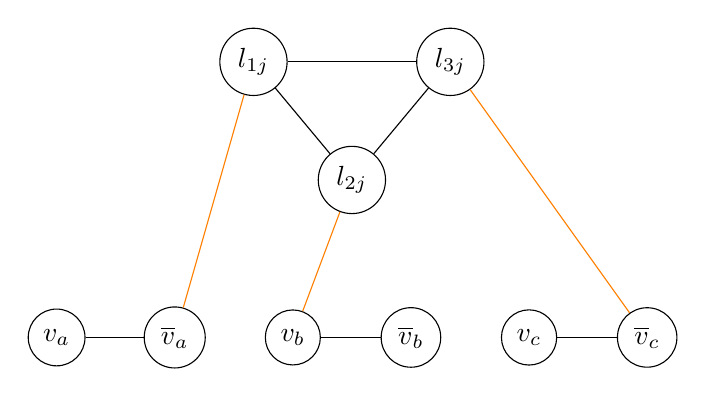
\begin{tikzpicture}
            \begin{scope}[every node/.style={circle, draw}]

                \node (va) at (0,0) {$v_a$};
                \node (nva) at (1.5,0) {$\overline{v}_a$};
                \path (va) edge (nva);

                \node (vb) at (3,0) {$v_b$};
                \node (nvb) at (4.5,0) {$\overline{v}_b$};
                \path (vb) edge (nvb);

                \node (vc) at (6,0) {$v_c$};
                \node (nvc) at (7.5,0) {$\overline{v}_c$};
                \path (vc) edge (nvc);

                \node (l2) at (3.75,2) {$l_{2j}$};
                \node (l1) at (2.5,3.5) {$l_{1j}$};
                \node (l3) at (5,3.5) {$l_{3j}$};
                \path (l1) edge (l2);
                \path (l2) edge (l3);
                \path (l3) edge (l1);

                \path[draw=orange] (l1) edge (nva);
                \path[draw=orange] (l2) edge (vb);
                \path[draw=orange] (l3) edge (nvc);

            \end{scope}
        \end{tikzpicture}
        \caption{Schema of how to use triangle "gadgets" for a single clause $C_j$}
        \label{img:3sat-nc-construction}
    \end{figure}

    Consider an instance of $\TSAT$ and construct a graph as shown in $\autoref{img:3sat-nc-construction}$, e.g.
    for each variable $v_i$ construct an edge between nodes $v_i$ and $\overline{v}_i$, and
    for each clause $C_j$ construct a triangle $l_{1j}, l_{2j}, l_{3j}$. Now, connect each node
    of the triangle with the corresponding literal in the clause (the \textcolor{orange}{orange edges}).
    Using this construction, we want to proove that there is a node cover of size $n+2m$ iff the $\TSAT$ instance is valid.

    Suppose the $\TSAT$ instance is feasible. We use the $n$ nodes of the feasible labeling corresponding to the literals.
    Now, because the labelling is valid, at least one orange edge per triangle must be covered, by construction.
    Therefore, we can choose $2$ additional nodes per triangle that cover the triangle and the remaining orange edges.

    On the other side, suppose there is a node cover of size (at most) $n+2m$.
    Analoguous, each triangle must have at least $2$ chosen nodes to cover each edge, and each literal-pair at least $1$ node,
    meaning our bounds must actually be exact to not overshoot $n+2m$. Therefore, the node cover represents a valid truth assignment,
    which is also a valid labelling, because each clause has a remaining orange edge, which is covered by
    one of the literals.

    Therefore, our reduction is Yes-preserving.
\end{proof}
\begin{remark}
    $\NC$ in bipartite graphs is in $\pP$.
\end{remark}
\begin{definition}[Independent set, $\IS$]
    For a graph $G= (N,E)$ we call $S \subset N$ a \vocab{independent set} (or \vocab{stable set}) if no edge has both nodes in $S$.
    The decision problem, called $\IS$, if there is a independent set of size at least $z$.
\end{definition}
\begin{theorem}
    $\IS \in \NPC$
\end{theorem}
\begin{proof}
    $\IS \in \NP$ trivial. We can also easily show that $C$ is a node cover iff $N \setminus C$ is stable.
\end{proof}
\begin{theorem}
    $\CLI \in \NPC$
\end{theorem}
\begin{proof}
    $\CLI \in \NP$ trivial. We can also easily show that $C$ is a clique in $G=(N,E)$ iff
    C is stable in $(N, \overline{E})$.
\end{proof}
\begin{definition}[Partition, $\PART$]
    Given $a_1,...,a_n \in \mathbb{Z^+}$. The decision problem if there is a set $S \subset \{1,...,n\}$ such that
    \begin{align*}
        \sum_{i \in S}a_i = \sum_{i \not \in S}a_i
    \end{align*}
    is called \vocab[partition]{partition problem}, $\PART$.
\end{definition}
\begin{theorem}
    $\PART \in \NPC$
\end{theorem}
\begin{sketch}
    We can show \cite[Ch.~15.5]{comb-optimization-korte}:
    \begin{align*}
        \SAT \redto \text{3-dim match} \redto \text{subset sum} \redto \PART
    \end{align*}
    %\footnote{see K+V 15.5}
\end{sketch}
\begin{remark}
    Still, $\PART$ has a pseudopolynomial algorithm using dynamic programming.
\end{remark}
\begin{definition}
    If a (numerical) problem is only $\NP$-complete if it is dependent on the size
    of the numbers (e.g. exponentially in count of numbers), we call it \vocab[NP-complete!weakly]{weakly $\NP$-complete}.
    Otherwise, we call it \vocab[NP-complete!strongly]{strongly $\NP$-complete}.
\end{definition}
\begin{definition}[3-partition, $\TPART$]
    Given the numbers $a_1,...,a_{3k} \in \integers$. The problem, if we can partition these numbers
    in sets of 3 such that every set has the same value, is called \vocab[partition!3-partition]{3-Partition}, or $\TPART$.
\end{definition}
\begin{theorem}
    $\TSAT$ is strongly $\NP$-complete.
\end{theorem}
\begin{proof}
    \todo{proof 3part NPC}
\end{proof}
\begin{remark}
    Only weakly $\NP$-complete problems could have pseudopolynomial algorithms (except $\pP = \NP$).
\end{remark}